% %%%%%%%%%%%%%%%%%%%%%%%%%%%%%%%%%%%%%%%%%%%%%%%%%%%%%%%%%%%%%%%%%%%%%%%%%%%%%%%%%
% حق نشر 1392-1402 دانش پژوهان ققنوس
% حقوق این اثر محفوظ است.
% 
% استفاده مجدد از متن و یا نتایج این اثر در هر شکل غیر قانونی است مگر اینکه متن حق
% نشر بالا در ابتدای تمامی مستندهای و یا برنامه‌های به دست آمده از این اثر
% بازنویسی شود. این کار باید برای تمامی مستندها، متنهای تبلیغاتی برنامه‌های
% کاربردی و سایر مواردی که از این اثر به دست می‌آید مندرج شده و در قسمت تقدیر از
% صاحب این اثر نام برده شود.
% 
% نام گروه دانش پژوهان ققنوس ممکن است در محصولات به در آمده شده از این اثر درج
% نشود که در این حالت با مطالبی که در بالا اورده شده در تضاد نیست. برای اطلاع
% بیشتر در مورد حق نشر آدرس زیر مراجعه کنید:
% 
% http://dpq.co.ir/licence
% %%%%%%%%%%%%%%%%%%%%%%%%%%%%%%%%%%%%%%%%%%%%%%%%%%%%%%%%%%%%%%%%%%%%%%%%%%%%%%%%%
% 
% در این بخص یک توصیف کوتا از محصول آورده می‌شود. این توصیف نباید از جمله‌های
% طولانی استفاده کند و خواننده را خسته نکند. در این بخش به موارد زیر پرداخته شود:
% 
% 1-    هدف ارائه این محصول چیست
% 2-    زمینه‌های کاربردی محصول چیست و چه منافعی برای کاربر دارد
% 
% \section{مقدمه}

رله کنترل از راه دور یک دستگاه الکترونیکی برای کنترل سایر دستگاه‌هایی است که با
انرژی الکتریکی کار می‌کنند.
برای نمونه درب‌های برقی با مجهز شدن به این دستگاه قابلیت کنترل از راه دور را
خواهند داشت.
گرچه این دستگاه برای کنترل درهای برقی به کار گرفته می‌شوند اما کاربرد آنها تنها
به این محدود نمی‌شود.

استفاده از این دستگاه برای کنترل سیستم‌هایی که دسترسی به آنها دشوار است بسیار
مناسب است.
این در حالی است که هزینه راه‌اندازی دستگاه بسیار کم بوده و مصرف توان آن بسیار
اندک است.
هزینه پایین این دستگاه یکی از ویژگی‌ها منحصر به فرد آن است.

از جمله مزیت‌های این دستگاه می‌توان به موارد زیر اشاره کرد:
\begin{itemize}
  \item هزینه پایین
  \item مصرف کم توان
  \item طول عمر بالا
  \item قابلیت مدیریت بیش از ۱۰۰ دستگاه ریموت
  \item پنل تعبیه شده برای کاربری در محل
  \item یک سال گارانتی محصول
\end{itemize}

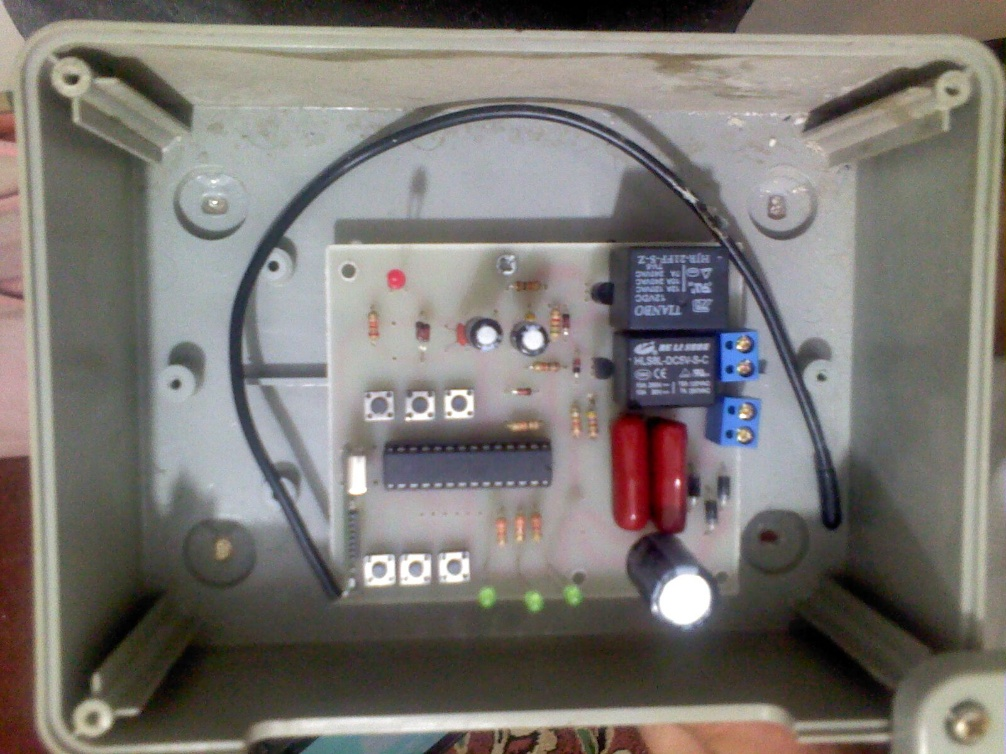
\includegraphics[width=0.8\textwidth]{image/view}

لازم به ذکر است که این دستگاه به صورت کامل در داخل کشور طراحی و تولید شده است.
